%%%%%%%%%%%%%%%%%%%%%%%%%%%%%%%%%%%%%%%%%%%%%%%%%%%%%%%%%%%%%%%
%% OXFORD THESIS TEMPLATE

% Use this template to produce a standard thesis that meets the Oxford University requirements for DPhil submission
%
% Originally by Keith A. Gillow (gillow@maths.ox.ac.uk), 1997
% Modified by Sam Evans (sam@samuelevansresearch.org), 2007
% Modified by John McManigle (john@oxfordechoes.com), 2015
%
% This version Copyright (c) 2015-2017 John McManigle
%
% Broad permissions are granted to use, modify, and distribute this software
% as specified in the MIT License included in this distribution's LICENSE file.
%

% I've (John) tried to comment this file extensively, so read through it to see how to use the various options.  Remember
% that in LaTeX, any line starting with a % is NOT executed.  Several places below, you have a choice of which line to use
% out of multiple options (eg draft vs final, for PDF vs for binding, etc.)  When you pick one, add a % to the beginning of
% the lines you don't want.


%%%%% CHOOSE PAGE LAYOUT
% The most common choices should be below.  You can also do other things, like replacing "a4paper" with "letterpaper", etc.

% This one will format for two-sided binding (ie left and right pages have mirror margins; blank pages inserted where needed):
\documentclass[a4paper,twoside]{ociamthesis}
% This one will format for one-sided binding (ie left margin > right margin; no extra blank pages):
%\documentclass[a4paper]{ociamthesis}
% This one will format for PDF output (ie equal margins, no extra blank pages):
%\documentclass[a4paper,nobind]{ociamthesis} 



%%%%% SELECT YOUR DRAFT OPTIONS
% Three options going on here; use in any combination.  But remember to turn the first two off before
% generating a PDF to send to the printer!

% This adds a "DRAFT" footer to every normal page.  (The first page of each chapter is not a "normal" page.)
\fancyfoot[C]{\emph{DRAFT Printed on \today}}  

% This highlights (in blue) corrections marked with (for words) \mccorrect{blah} or (for whole
% paragraphs) \begin{mccorrection} . . . \end{mccorrection}.  This can be useful for sending a PDF of
% your corrected thesis to your examiners for review.  Turn it off, and the blue disappears.
\correctionstrue


%%%%% BIBLIOGRAPHY SETUP
% Note that your bibliography will require some tweaking depending on your department, preferred format, etc.
% The options included below are just very basic "sciencey" and "humanitiesey" options to get started.
% If you've not used LaTeX before, I recommend reading a little about biblatex/biber and getting started with it.
% If you're already a LaTeX pro and are used to natbib or something, modify as necessary.
% Either way, you'll have to choose and configure an appropriate bibliography format...

% The science-type option: numerical in-text citation with references in order of appearance.
\usepackage[style=numeric-comp, sorting=none, backend=biber, doi=false, isbn=false]{biblatex}
\newcommand*{\bibtitle}{References}

% The humanities-type option: author-year in-text citation with an alphabetical works cited.
%\usepackage[style=authoryear, sorting=nyt, backend=biber, maxcitenames=2, useprefix, doi=false, isbn=false]{biblatex}
%\newcommand*{\bibtitle}{Works Cited}

% This makes the bibliography left-aligned (not 'justified') and slightly smaller font.
\renewcommand*{\bibfont}{\raggedright\small}

% Change this to the name of your .bib file (usually exported from a citation manager like Zotero or EndNote).
\addbibresource{references.bib}


% Uncomment this if you want equation numbers per section (2.3.12), instead of per chapter (2.18):
%\numberwithin{equation}{subsection}



%%%%% THESIS / TITLE PAGE INFORMATION
% Everybody needs to complete the following:
\title{Search for a low-energy excess of electron neutrinos in MicroBooNE}
\author{Stefano Roberto Soleti}
\college{St Catherine's College}

% Master's candidates who require the alternate title page (with candidate number and word count)
% must also un-comment and complete the following three lines:
%\masterssubmissiontrue
%\candidateno{933516}
%\wordcount{28,815}

% Uncomment the following line if your degree also includes exams (eg most masters):
\renewcommand{\submittedtext}{A thesis submitted for the degree of}
% Your full degree name.  (But remember that DPhils aren't "in" anything.  They're just DPhils.)
\degree{Doctor of Philosophy}
% Term and year of submission, or date if your board requires (eg most masters)
\degreedate{Trinity 2019}


%%%%% YOUR OWN PERSONAL MACROS
% This is a good place to dump your own LaTeX macros as they come up.

% To make text superscripts shortcuts
	\renewcommand{\th}{\textsuperscript{th}} % ex: I won 4\th place
	\newcommand{\nd}{\textsuperscript{nd}}
	\renewcommand{\st}{\textsuperscript{st}}
	\newcommand{\rd}{\textsuperscript{rd}}

%%%%% THE ACTUAL DOCUMENT STARTS HERE
\begin{document}



%%%%% CHOOSE YOUR LINE SPACING HERE
% This is the official option.  Use it for your submission copy and library copy:
\setlength{\textbaselineskip}{22pt plus2pt}
% This is closer spacing (about 1.5-spaced) that you might prefer for your personal copies:
%\setlength{\textbaselineskip}{18pt plus2pt minus1pt}

% You can set the spacing here for the roman-numbered pages (acknowledgements, table of contents, etc.)
\setlength{\frontmatterbaselineskip}{17pt plus1pt minus1pt}

% Leave this line alone; it gets things started for the real document.
\setlength{\baselineskip}{\textbaselineskip}


%%%%% CHOOSE YOUR SECTION NUMBERING DEPTH HERE
% You have two choices.  First, how far down are sections numbered?  (Below that, they're named but
% don't get numbers.)  Second, what level of section appears in the table of contents?  These don't have
% to match: you can have numbered sections that don't show up in the ToC, or unnumbered sections that
% do.  Throughout, 0 = chapter; 1 = section; 2 = subsection; 3 = subsubsection, 4 = paragraph...

% The level that gets a number:
\setcounter{secnumdepth}{2}
% The level that shows up in the ToC:
\setcounter{tocdepth}{2}


%%%%% ABSTRACT SEPARATE
% This is used to create the separate, one-page abstract that you are required to hand into the Exam
% Schools.  You can comment it out to generate a PDF for printing or whatnot.
\begin{abstractseparate}
	The Micro Booster Neutrino Experiment (MicroBooNE) is a Liquid Argon Time Projection Chamber (LArTPC) designed for short-baseline neutrino physics at the Fermi National Accelerator Laboratory. The main physics goal of MicroBooNE is to address the low-energy excess of electron-like events observed by the MiniBooNE experiment and, if confirmed, clarify its nature.
The MiniBooNE experiment is a Cherenkov detector and this technology does not allow to distinguish between electrons and single photons in the final state. 
LArTPC detectors, instead, offer excellent granularity and powerful separation between electrons and photons. For this reason, they represent an ideal technology for the detection of electron neutrino interactions.
This thesis presents the first fully-automated electron neutrino selection in a LArTPC. The selection looks for charged-current electron neutrino interactions with no pions and at least one proton in the final state. It is applied on a sub-sample of the data acquired by the detector in the Booster Neutrino Beam, corresponding to $4.34\times10^{19}$~protons-on-target. A validation of the analysis is performed on two orthogonal side-bands, enriched with neutral-current and charged-current muon neutrino interactions, respectively. The uncertainties on the neutrino cross sections, flux, and detector simulation are evaluated.
The MicroBooNE detector is placed off-axis with the Neutrinos at the Main Injector (NuMI) beam. An independent dataset of events acquired by triggering on the NuMI beam is employed to measure the significance of the detection of electron neutrinos in the beam using the selection presented here. 
The sensitivity of the MicroBooNE experiment to the MiniBooNE low-energy excess of electron-like events is evaluated. The efficiency and background-rejection power necessary to achieve $5\sigma$ sensitivity are also quantified. % Create an abstract.tex file in the 'text' folder for your abstract.
\end{abstractseparate}


% JEM: Pages are roman numbered from here, though page numbers are invisible until ToC.  This is in
% keeping with most typesetting conventions.
\begin{romanpages}

% Title page is created here
\maketitle

%%%%% DEDICATION -- If you'd like one, un-comment the following.
%\begin{dedication}
%This thesis is dedicated to\\
%someone\\
%for some special reason\\
%\end{dedication}

%%%%% ACKNOWLEDGEMENTS -- Nothing to do here except comment out if you don't want it.
\begin{acknowledgements}
 	
This is where you thank your advisor, colleagues, and family and friends.

Lorem ipsum dolor sit amet, consectetur adipiscing elit. Vestibulum feugiat et est at accumsan. Praesent sed elit mattis, congue mi sed, porta ipsum. In non ullamcorper lacus. Quisque volutpat tempus ligula ac ultricies. Nam sed erat feugiat, elementum dolor sed, elementum neque. Aliquam eu iaculis est, a sollicitudin augue. Cras id lorem vel purus posuere tempor. Proin tincidunt, sapien non dictum aliquam, ex odio ornare mauris, ultrices viverra nisi magna in lacus. Fusce aliquet molestie massa, ut fringilla purus rutrum consectetur. Nam non nunc tincidunt, rutrum dui sit amet, ornare nunc. Donec cursus tortor vel odio molestie dignissim. Vivamus id mi erat. Duis porttitor diam tempor rutrum porttitor. Lorem ipsum dolor sit amet, consectetur adipiscing elit. Sed condimentum venenatis consectetur. Lorem ipsum dolor sit amet, consectetur adipiscing elit.

\end{acknowledgements}

%%%%% ABSTRACT -- Nothing to do here except comment out if you don't want it.
\begin{abstract}
	The Micro Booster Neutrino Experiment (MicroBooNE) is a Liquid Argon Time Projection Chamber (LArTPC) designed for short-baseline neutrino physics at the Fermi National Accelerator Laboratory. The main physics goal of MicroBooNE is to address the low-energy excess of electron-like events observed by the MiniBooNE experiment and, if confirmed, clarify its nature.
The MiniBooNE experiment is a Cherenkov detector and this technology does not allow to distinguish between electrons and single photons in the final state. 
LArTPC detectors, instead, offer excellent granularity and powerful separation between electrons and photons. For this reason, they represent an ideal technology for the detection of electron neutrino interactions.
This thesis presents the first fully-automated electron neutrino selection in a LArTPC. The selection looks for charged-current electron neutrino interactions with no pions and at least one proton in the final state. It is applied on a sub-sample of the data acquired by the detector in the Booster Neutrino Beam, corresponding to $4.34\times10^{19}$~protons-on-target. A validation of the analysis is performed on two orthogonal side-bands, enriched with neutral-current and charged-current muon neutrino interactions, respectively. The uncertainties on the neutrino cross sections, flux, and detector simulation are evaluated.
The MicroBooNE detector is placed off-axis with the Neutrinos at the Main Injector (NuMI) beam. An independent dataset of events acquired by triggering on the NuMI beam is employed to measure the significance of the detection of electron neutrinos in the beam using the selection presented here. 
The sensitivity of the MicroBooNE experiment to the MiniBooNE low-energy excess of electron-like events is evaluated. The efficiency and background-rejection power necessary to achieve $5\sigma$ sensitivity are also quantified.
\end{abstract}

%%%%% MINI TABLES
% This lays the groundwork for per-chapter, mini tables of contents.  Comment the following line
% (and remove \minitoc from the chapter files) if you don't want this.  Un-comment either of the
% next two lines if you want a per-chapter list of figures or tables.
\dominitoc % include a mini table of contents
%\dominilof  % include a mini list of figures
%\dominilot  % include a mini list of tables

% This aligns the bottom of the text of each page.  It generally makes things look better.
\flushbottom

% This is where the whole-document ToC appears:
\tableofcontents

\listoffigures
	\mtcaddchapter
% \mtcaddchapter is needed when adding a non-chapter (but chapter-like) entity to avoid confusing minitoc

% Uncomment to generate a list of tables:
%\listoftables
%	\mtcaddchapter

%%%%% LIST OF ABBREVIATIONS
% This example includes a list of abbreviations.  Look at text/abbreviations.tex to see how that file is
% formatted.  The template can handle any kind of list though, so this might be a good place for a
% glossary, etc.
% First parameter can be changed eg to "Glossary" or something.
% Second parameter is the max length of bold terms.
\begin{mclistof}{List of Abbreviations}{3.2cm}

\item[BSM] Beyond the Standard Model of particle physics
\item[V-A] Vector - Axial current in the electroweak interaction
\item[PMNS] Pontecorvo–Maki–Nakagawa–Sakata mixing matrix of the neutrino sector
\item[MSW] Mikheyev-Smirnov-Wolfenstein effect, also called \emph{matter effect}
\item[LSND] Liquid Scintillator Neutrino Detector, neutrino detection experiment at Los Alamos
\item[LEP] Large Electron-Positron Collider at CERN
\item[GUT] Grand Unification Theory
\item[BNB] Booster Neutrino Beam at Fermilab
\item[PMT] Photomultiplier Tube
\item[FSI] Final State Interactions 
\item[CCQE] Charged-Current Quasi-Elastic interaction
\item[CCRES] Charged-Current Resonant interaction
\item[CCDIS] Charged-Current Deep Inelastic Scattering
\item[DAR] Decay-at-rest
\item[DIF] Decay-in-flight
\item[MiniBooNE] Mini Booster Neutrino Experiment
\item[KARMEN] Karlsruhe Rutherford Medium Energy Neutrino experiment
\item[MicroBooNE] Micro Booster Neutrino Experiment
\item[OPERA] Oscillation Project with Emulsion-Tracking Apparatus experiment
\item[LArTPC] Liquid Argon Time Projection Chamber
\item[NC] Neutral Current interaction
\item[CC] Charged Current interaction
\item[SciBooNE] SciBar Booster Neutrino Experiment
\item[DUNE] Deep Underground Neutrino Experiment
\item[CNGS] CERN Neutrinos to Gran Sasso
\item[ArgoNeuT] Argon Neutrino Test
\item[ICARUS] Imaging Cosmic And Rare Underground Signal
\item[SNEWS] SuperNova Early Warning System
\end{mclistof} 


% The Roman pages, like the Roman Empire, must come to its inevitable close.
\end{romanpages}


%%%%% CHAPTERS
% Add or remove any chapters you'd like here, by file name (excluding '.tex'):
\flushbottom
\begin{savequote}[8cm]
 Secondo la proposta di Pauli si può, ad esempio, ammettere l'esistenza di una nuova particella, il così detto neutrino avente carica elettrica nulla e massa dell'ordine di grandezza di quella dell'elettrone o minore.
 \qauthor{--- Enrico Fermi \cite{Fermi:1933jpa}}
\end{savequote}

\chapter{\label{ch:1-intro}Introduction} 

This thesis describes the first fully-automated electron neutrino search in a Liquid Argon Time Projection Chamber (LArTPC) and the work towards the search for a low-energy excess of electron neutrinos at MicroBooNE.

The history of neutrinos begins with an anomaly: the continuous energy spectrum of the nuclear beta decay could not be explained with a two-body decay. It took more than 25 years to experimentally confirm their existence, but neutrinos continued to puzzle experimentalists until the early 2000, when the existence of neutrino oscillations was finally settled. 
However, in the last two decades, several experiments collected results not fully agreement with a 3-generation scenario.
In particular, LSND first, and MiniBooNE later, found an excess of electron neutrinos compatible with the existence of a fourth, non weakly-interacting, neutrino. The goal of the MicroBooNE experiment is to definitely clarify the nature of the excess.

In \textbf{Chapter \ref{ch:2-neutrinophysics}} we will provide a brief theoretical introduction to the theory of neutrino oscillations and to the main experimental techniques employed to detected them.
In \textbf{Chapter \ref{ch:3-anomalies}}, the LSND and MiniBooNE experiment will be described. A brief overview of other anomalous results and their possible theoretical interpretations will also be provided.
The MicroBooNE experiment will be described in \textbf{Chapter \ref{ch:4-microboone}}. We will enumerate the physics goals of the experiment and explain the main features of the detector, with an overview of the artificial neutrino beams at Fermilab.
The techniques employed to reconstruct the signals coming from the detector will be described in \textbf{Chapter \ref{sec:eventreco}}. The pattern recognition is performed by the Pandora framework, which will be briefly outlined.
\textbf{Chapter \ref{ch:6-analysis}} will thoroughly describe the fully automated electron-neutrino selection and its validation, performed with a study on side-bands and on an independent data sample. The systematic uncertainties in the selection will be estimated in \textbf{Chapter \ref{sec:systematics}}.
In \textbf{Chapter \ref{sec:sensitivity}} the sensitivity to the low-energy excess of the MiniBooNE experiment in the electron hypothesis will be evaluated. The performances required to reach a $5\sigma$ sensitivity will also be estimated.
The thesis ends in \textbf{Chapter \ref{ch:7-conclusions}} with a summary of the results and an overview of the future prospects for MicroBooNE and for the sterile neutrino searches in general. 

\vspace{1em}

\textbf{Appendix \ref{sec:mucs}} contains a publication, whose corresponding author is the author of this thesis, with the first measurement of the cosmic-ray reconstruction efficiency in a LArTPC.
\begin{savequote}[8cm]
Alles Gescheite ist schon gedacht worden.\\
Man muss nur versuchen, es noch einmal zu denken.

All intelligent thoughts have already been thought;\\
what is necessary is only to try to think them again.
  \qauthor{--- Johann Wolfgang von Goethe \cite{von_goethe_wilhelm_1829}}
\end{savequote}

\chapter{\label{ch:2-litreview}Background}

\minitoc

\section{Introduction}

This document introduction won't serve as a complete primer on \LaTeX.  There are plenty of those online, and googling your questions will often get you answers, especially from \url{http://tex.stackexchange.com}.

Instead, let's talk a little about a few of the features and packages lumped into this template situation.  The \verb|savequote| environment at the beginning of chapters can add some wittiness to your thesis.  If you don't like the quotes, just remove that block.

For when it comes time to do corrections, there are two useful commands here.  First, the \verb|mccorrect| command allows you to highlight a short correction \mccorrect{like this one}.  When the thesis is typeset normally, the correction will just appear as part of the text.  However, when you declare \verb|\correctionstrue| in the main \verb|Oxford_Thesis.tex| file, that correction will be highlighted in blue.  That might be useful for submitting a post-viva, corrected copy to your examiners so they can quickly verify you've completed the task.

\begin{mccorrection}
For larger chunks, like this paragraph or indeed entire figures, you can use the \verb|mccorrection| environment.  This environment highlights paragraph-sized and larger blocks with the same blue colour.
\end{mccorrection}

Read through the \verb|Oxford_Thesis.tex| file to see the various options for one- and two-sided printing, including or excluding the separate abstract page, and turning corrections and draft footer on or off, and the separate option to centre your text on the page (for PDF submission) or offset it (for binding).  There is also a separate option for master's degree submissions, which changes identifying information to candidate number and includes a word count.  (Unfortunately, \LaTeX has a hard time doing word counts automatically, so you'll have to enter the count manually if you require this.)

\section{Cardiac Imaging}\label{app:imaging}

Within months of Röntgen's discovery of the X-ray in \mccorrect{1895}\cite{gagliardi_rontgen_1996}, cardiac pathology was being investigated via non-invasive imaging \cite{gagliardi_cardiac_1996}.  Over the intervening years, cardiac imaging modalities and techniques have advanced significantly.  Clinically, cardiac imaging is used for two broad purposes: diagnosis of pathophysiology and guidance of interventional procedures.  These applications impose different requirements on imaging equipment, image acquisition time, computational complexity, spatial and temporal resolution, and tissue discrimination.  The common diagnostic and interventional cardiac imaging techniques in current clinical practice are reviewed below.  An accessible introduction to the physics of medical imaging can be found in Webb's \textit{Introduction to Biomedical Imaging} \cite{webb_introduction_2002}.  A comprehensive overview of the use of imaging in clinical cardiology is presented in Leeson's \textit{Cardiovascular Imaging} \cite{leeson_cardiovascular_2011}.

\subsection{Diagnostic Imaging}
\label{sub:diagnostic}

Beyond the chest X-ray (`plain film'), the key non-invasive imaging modalities in diagnostic cardiology are echocardiography, magnetic resonance imaging, and X-ray computed tomography, which are reviewed below.  Nuclear medicine, including positron emission tomography (PET) and single-photon emission computed tomography (SPECT), are not discussed here, as they do not play a role in the chapters to follow.

\subsubsection{Echocardiography}

\begin{figure}
\centering\includegraphics[width=0.7\textwidth]{figures/sample/Gray498.png} 
\caption[Four-chamber illustration of the human heart.]{Four-chamber illustration of the human heart.  Clockwise from upper-left: right atrium, left atrium, left ventricle, right ventricle.}
\label{fig:fourchamber}\end{figure}

The use of acoustic waves for medical diagnosis, inspired by naval sonar, was initially developed in the 1940s \cite{gagliardi_ultrasonography_1996}.  By 1954, the first clinically useful cardiac ultrasound -- examining motion of the mitral valve in stenosis -- was reported \cite{edler_ultrasonic_1957}.  These early scans were one-dimensional images (`A-mode'), sometimes repeated to generate a time axis (`M-mode').   The sector-scanning probe was developed in the 1970s \cite{bom_ultrasonic_1971,griffith_sector_1974}, leading to the `B-mode' that a modern cardiologist would recognise as an echocardiogram.



%% APPENDICES %% 
% Starts lettered appendices, adds a heading in table of contents, and adds a
%    page that just says "Appendices" to signal the end of your main text.
\startappendices
% Add or remove any appendices you'd like here:

\chapter{Measurement of cosmic-ray reconstruction efficiencies in the MicroBooNE LArTPC using a small external cosmic-ray counter}
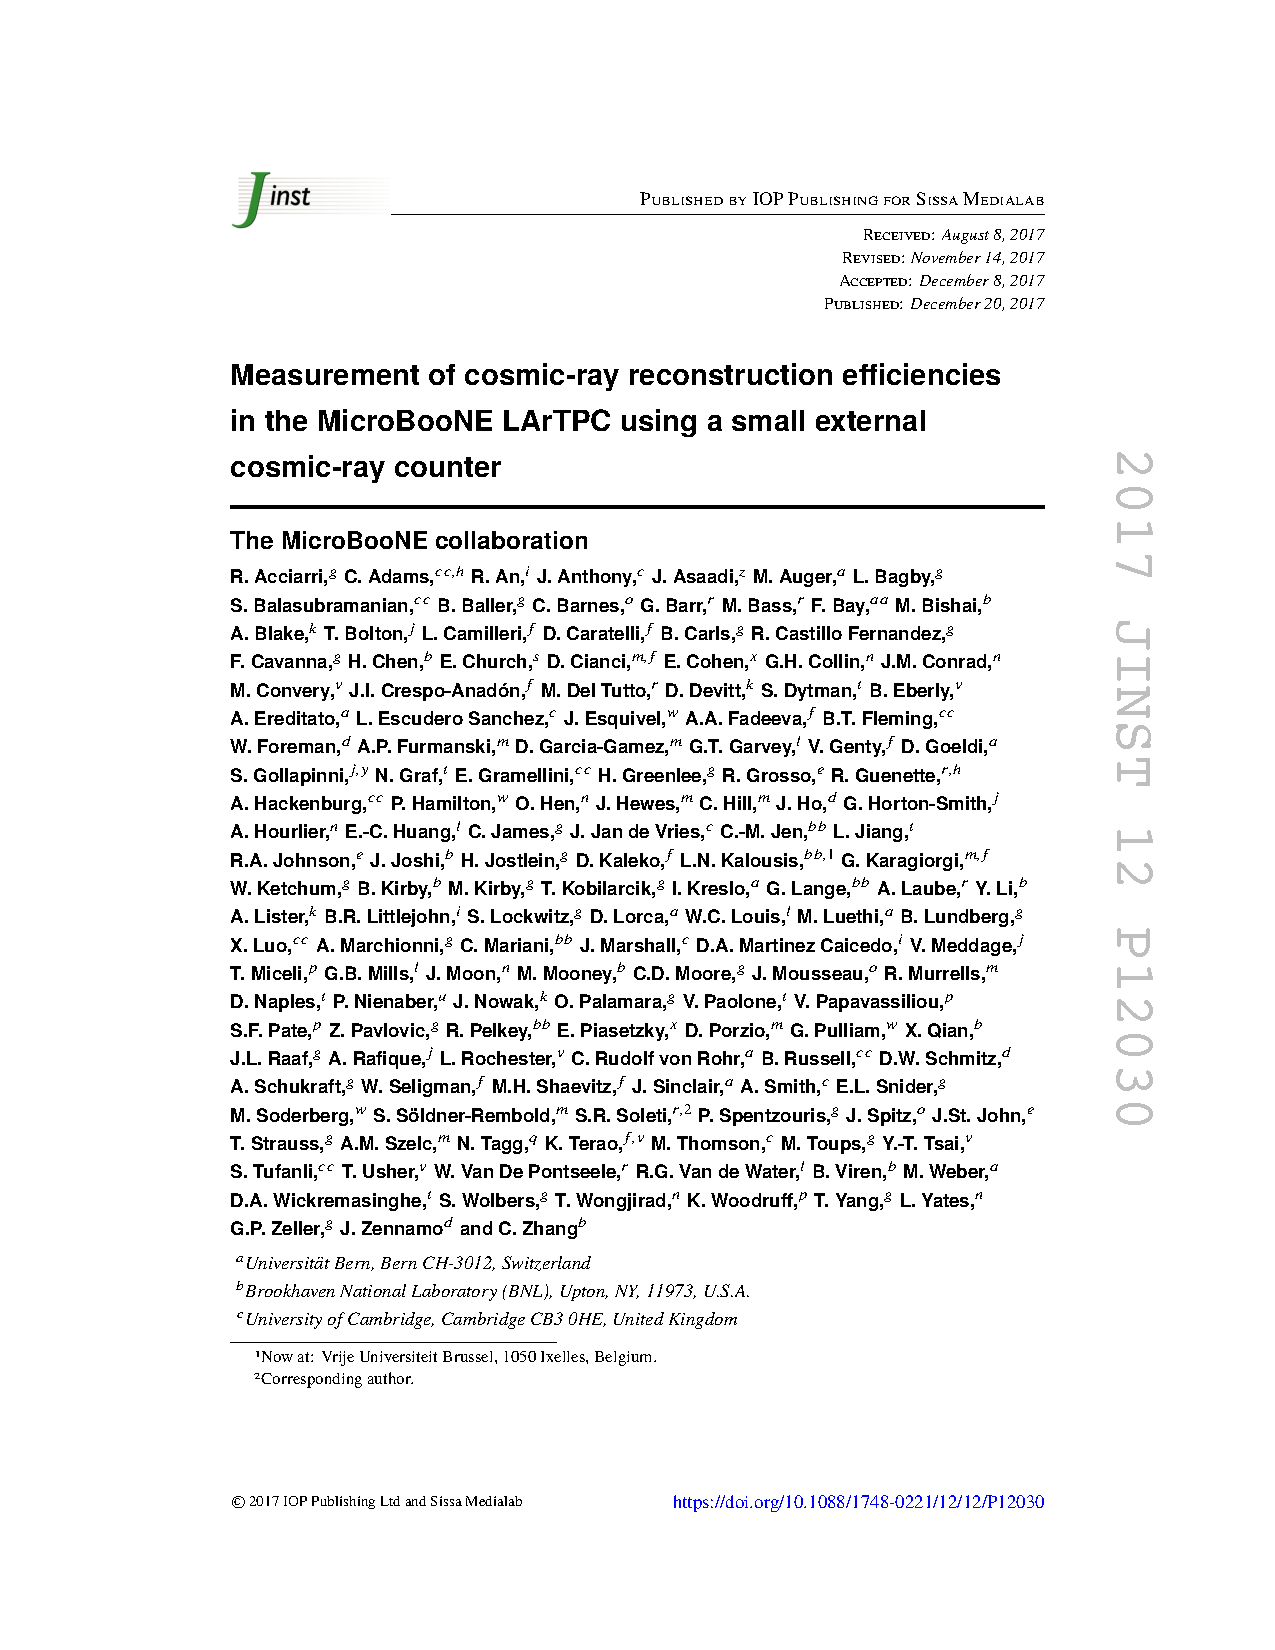
\includepdf[pages=-,pagecommand={},width=1.45\textwidth]{figures/cosmic_paper.pdf}



%%%%% REFERENCES

% JEM: Quote for the top of references (just like a chapter quote if you're using them).  Comment to skip.
\begin{savequote}[8cm]
The first kind of intellectual and artistic personality belongs to the hedgehogs, the second to the foxes \dots
  \qauthor{--- Sir Isaiah Berlin \cite{berlin_hedgehog_2013}}
\end{savequote}

\setlength{\baselineskip}{0pt} % JEM: Single-space References

{\renewcommand*\MakeUppercase[1]{#1}%
\printbibliography[heading=bibintoc,title={\bibtitle}]}


\end{document}
